\documentclass[8pt,apectratio=169]{beamer}

\usetheme[progressbar=frametitle]{metropolis}
\usepackage{appendixnumberbeamer}
\usepackage[style=authoryear, backend=bibtex8, natbib=true, maxcitenames=2]{biblatex}

\usepackage[utf8]{inputenc} % utf8x  defines more symbols, but may cause compatible problems
\usepackage{lmodern,textcomp} % Latin Modern fonts, contains €

\usepackage{graphicx}
\usepackage{import}

\usepackage{booktabs}
\usepackage[scale=2]{ccicons}

\usepackage{pgfplots}
\usepgfplotslibrary{dateplot}

\usepackage{xspace}
\newcommand{\themename}{\textbf{\textsc{metropolis}}\xspace}

% Math
\usepackage{amsmath}
\usepackage{bm} % bold symbol in math mode

% Optional packages
\usepackage{xcolor}
\usepackage{multicol}
\usepackage{hyperref}
\usepackage[super,negative]{nth} % allows writing 1st, 2nd, 3rd with superscript
\usepackage{ulem} % use the "sout" tag to "strikethrough" text
\usepackage{tcolorbox}

% Select what to do with command \comment:
  % \newcommand{\comment}[1]{}  %comments not shown
  % \newcommand{\comment}[1]{\par {\bfseries \color{blue} #1 \par}} %comments shown
% Select what to do with todonotes: i.e. \todo{}, \todo[inline]{}
  % \usepackage[disable]{todonotes} % notes not shown
  % \usepackage[draft]{todonotes}   % notes shown

%\numberwithin{equation}{section}

%\addbibresource{references}

\titlegraphic{\hfill 
\includegraphics[width=0.15 \textwidth]{figures/logo}}
\title{Microeconomics III, Ex. Class 4: Problem Set 1\footnote{Slides created for exercise class 4, with reservation for possible errors.\\}}
\author{Thor Donsby Noe (\href{mailto:thor.noe@econ.ku.dk}{thor.noe@econ.ku.dk})}
\date{September 11 2019} % \today
\institute{\normalsize Department of Economics, University of Copenhagen}

    % \definecolor{BlueTOL}{HTML}{222255}
    \definecolor{BrownTOL}{HTML}{666633}
    \definecolor{GreenTOL}{HTML}{225522}
    % \setbeamercolor{normal text}{fg=BlueTOL,bg=white}
    \setbeamercolor{alerted text}{fg=BrownTOL}
    \setbeamercolor{example text}{fg=GreenTOL}
    \setbeamercolor{background canvas}{bg=white}

    \setbeamercolor{block title alerted}{use=alerted text,
        fg=alerted text.fg,
        bg=alerted text.bg!80!alerted text.fg}
    \setbeamercolor{block body alerted}{use={block title alerted, alerted text},
        fg=alerted text.fg,
        bg=block title alerted.bg!50!alerted text.bg}
    \setbeamercolor{block title example}{use=example text,
        fg=example text.fg,
        bg=example text.bg!80!example text.fg}
    \setbeamercolor{block body example}{use={block title example, example text},
        fg=example text.fg,
        bg=block title example.bg!50!example text.bg}

\begin{document}
\maketitle

% ------------------------------------------------------------------------------
% ------ FRAME -----------------------------------------------------------------
% ------------------------------------------------------------------------------
\begin{frame}{Outline}
    \tableofcontents
\end{frame}

\section{PS4, Ex. 1 (A): MSNE and best-response functions}

\begin{frame}{Kahoot: PS4, Ex. 1 (A): MSNE and best-response functions}
  Form a group for each table:
  \begin{itemize}
    \item Get prepared to answer exercise 1 in problem set 4 as a team (5 min).
  \end{itemize}
  
\includegraphics[width=\textwidth]{figures/kahoot}
\end{frame}
\begin{frame}{PS4, Ex. 1 (A): MSNE and best-response functions}
  Find all equilibria (pure and mixed) in the following games, first analytically and then through plotting the best-response functions.
  \begin{multicols}{2}
    \begin{itemize}
      \item[(a)]
    \end{itemize}
    \begin{table}
      \begin{tabular}{cl|c|c|}
          & \multicolumn{1}{c}{} & \multicolumn{2}{c}{Player 2}\\
          \parbox[t]{1mm}{\multirow{3}{*}{\rotatebox[origin=r]{90}{Player 1}}}
          & \multicolumn{1}{c}{} & \multicolumn{1}{c}{L (q)} & \multicolumn{1}{c}{L (1-q)} \\\cline{3-4}
          & T (p) & 3, 3 & 0, 0 \\\cline{3-4}
          & B (1-p) & 0, 0 & 4, 4 \\\cline{3-4}
      \end{tabular}
    \end{table}
  \vfill\null \columnbreak
    \begin{itemize}
      \item[(b)]
    \end{itemize}
    \begin{table}
      \begin{tabular}{cl|c|c|}
          & \multicolumn{1}{c}{} & \multicolumn{2}{c}{Player 2}\\
          \parbox[t]{1mm}{\multirow{3}{*}{\rotatebox[origin=r]{90}{Player 1}}}
          & \multicolumn{1}{c}{} & \multicolumn{1}{c}{L (q)} & \multicolumn{1}{c}{L (1-q)} \\\cline{3-4}
          & T (p) & 1, 1 & 0, 0 \\\cline{3-4}
          & B (1-p) & 1, 0 & 2, 1 \\\cline{3-4}
      \end{tabular}
    \end{table}
  \vfill\null
  \end{multicols}
\end{frame}
\begin{frame}{PS4, Ex. 1.a (A): MSNE and best-response functions}
  \begin{multicols}{2}
    \begin{itemize}
      \item[(a)] Find all equilibria (pure and mixed), first analytically and then through plotting the BR functions.
    \end{itemize}
    \begin{table}
      \begin{tabular}{cl|c|c|}
        & \multicolumn{1}{c}{} & \multicolumn{2}{c}{\color{blue}Player 2}\\
        \parbox[t]{1mm}{\multirow{3}{*}{\rotatebox[origin=r]{90}{\color{red}Player 1}}}
        & \multicolumn{1}{c}{} & \multicolumn{1}{c}{L (q)} & \multicolumn{1}{c}{L (1-q)} \\\cline{3-4}
        & T (p) & \textcolor{red}{3}, \textcolor{blue}{3} & 0, 0 \\\cline{3-4}
        & B (1-p) & 0, 0 & \textcolor{red}{4}, \textcolor{blue}{4} \\\cline{3-4}
      \end{tabular}
    \end{table}
    Find $q$ such that Player 1 expect to have equal payoffs from playing $T$ and $B$:
    \begin{align*}
      E[u_1|T]&=E[u_1|B]\\
      3q &= 4(1-q) \Rightarrow q = \frac{4}{7}
    \end{align*}
    The players have symmetric payoffs, thus:
    \begin{align*}
      NE=(p^{*},q^{*})=\left\{(0,0);(1,1);\left(\frac{4}{7},\frac{4}{7}\right)\right\}
    \end{align*}
  \vfill\null \columnbreak
    Plot the BR functions:
    \vspace{-8pt}
    \begin{align*}
      BR_1(q)=\left\{ \begin{array}{lcl}
          p=0       & \text{if} & q<4/7 \\
          p\in[0,1] & \text{if} & q=4/7 \\
          p = 1     & \text{if} & q>4/7
      \end{array}\right. \\
      BR_2(p)=\left\{ \begin{array}{lcl}
          q=0       & \text{if} & p<4/7  \\
          q\in[0,1] & \text{if} & p=4/7 \\
          q = 1     & \text{if} & p>4/7
      \end{array}\right.
    \end{align*}
    \vspace{-8pt}
    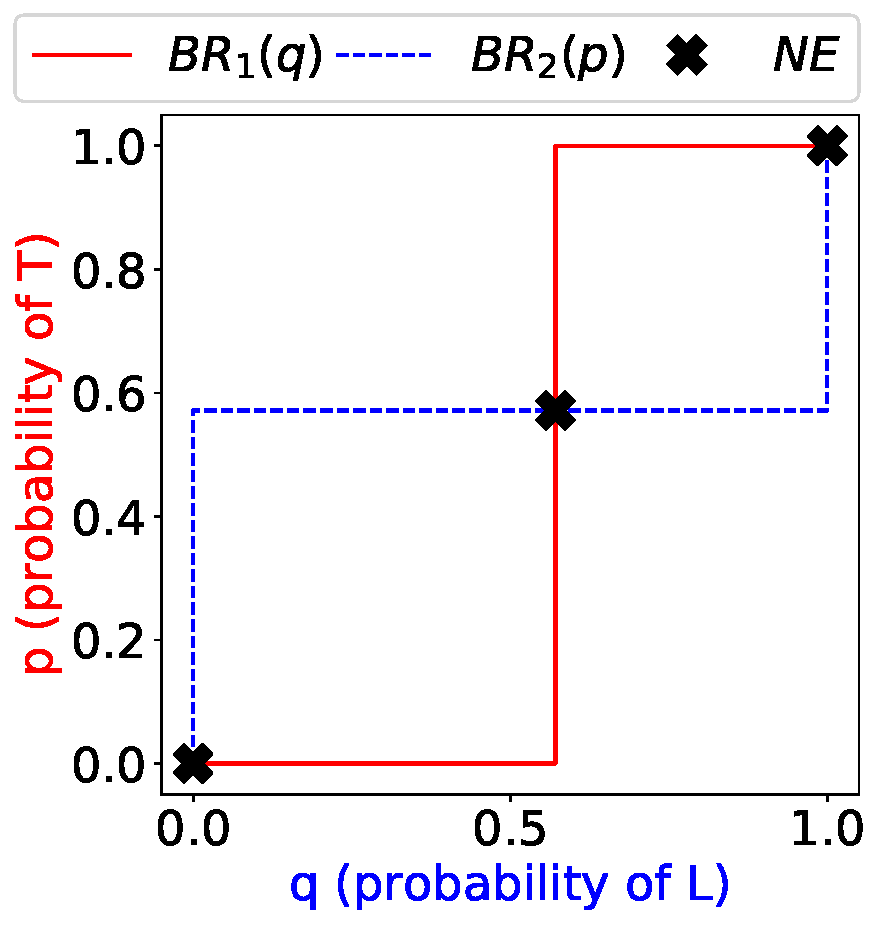
\includegraphics[width=\columnwidth]{figures/1a}
  \vfill\null
  \end{multicols}
\end{frame}
\begin{frame}{PS4, Ex. 1.b (A): MSNE and best-response functions}
  \begin{multicols}{2}
    \begin{itemize}
      \item[(b)] Find all NE, first analytically:
    \end{itemize}
    \begin{table}
      \begin{tabular}{cl|c|c|}
        & \multicolumn{1}{c}{} & \multicolumn{2}{c}{\color{blue}Player 2}\\
        \parbox[t]{1mm}{\multirow{3}{*}{\rotatebox[origin=r]{90}{\color{red}Player 1}}}
        & \multicolumn{1}{c}{} & \multicolumn{1}{c}{L (q)} & \multicolumn{1}{c}{L (1-q)} \\\cline{3-4}
        & T (p) & \textcolor{red}{1}, \textcolor{blue}{1} & 0, 0 \\\cline{3-4}
        & B (1-p) & \textcolor{red}{1}, 0 & \textcolor{red}{2}, \textcolor{blue}{1} \\\cline{3-4}
      \end{tabular}
    \end{table}
    Player 1 is indifferent for:
    \begin{align*}
      E[u_1|T]&=E[u_1|B]\\
      q &= q + 2(1-q) \Rightarrow q = 1
    \end{align*}
    Player 2 is indifferent for:
    \begin{align*}
      E[u_2|L]&=E[u_2|R]\\
      p &= 1-p \Rightarrow p = \frac{1}{2}
    \end{align*}
    The pure and mixed strategy NE are:
    \begin{align*}
      NE:\left\{(0,0);(1,1);\left(p\in\left[\frac{1}{2},1\right),q=1\right)\right\}
    \end{align*}
  \vfill\null \columnbreak
    Then through plotting the BR functions:
    \vspace{-8pt}
    \begin{align*}
      BR_1(q)=\left\{ \begin{array}{lcl}
          p=0       & \text{if} & q<1 \\
          p\in[0,1] & \text{if} & q=1
      \end{array}\right. \\
      BR_2(p)=\left\{ \begin{array}{lcl}
          q=0       & \text{if} & p<1/2  \\
          q\in[0,1] & \text{if} & p=1/2 \\
          q=1       & \text{if} & p>1/2
      \end{array}\right.
    \end{align*}
    \vspace{-8pt}
    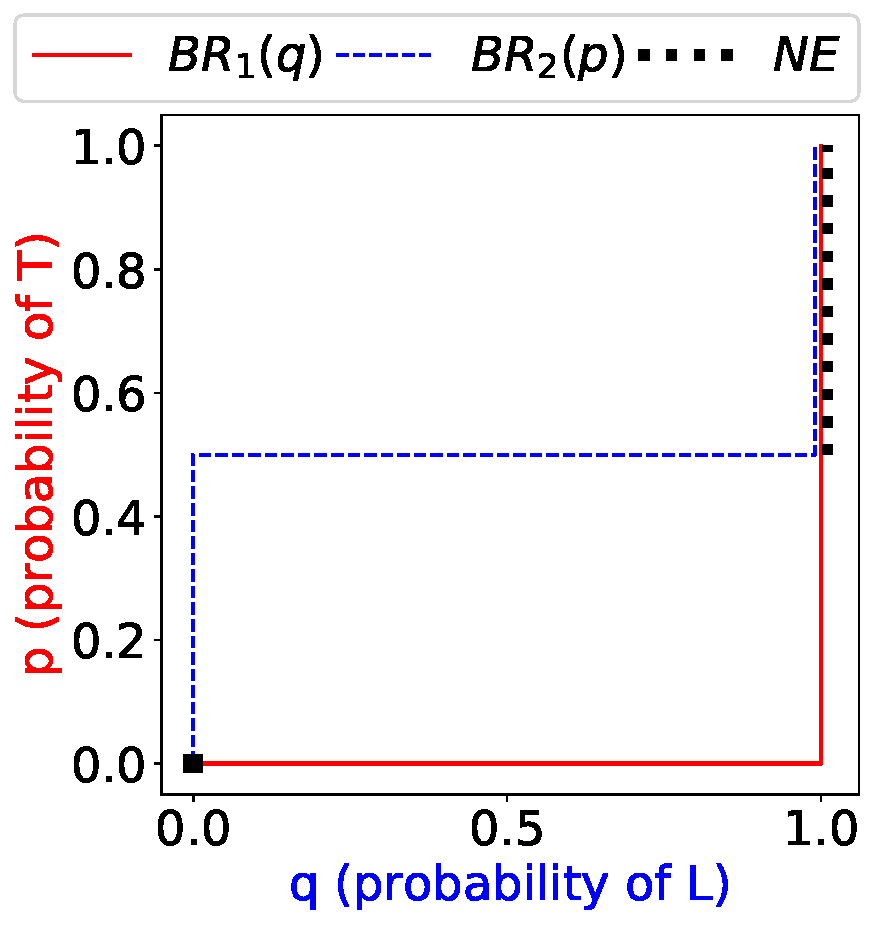
\includegraphics[width=\columnwidth]{figures/1b}
  \vfill\null
  \end{multicols}
\end{frame}


\section{PS4, Ex. 3: The Focal Point}

\begin{frame}{PS4, Ex. 3: The Focal Point}
  \begin{multicols}{2}
    Thomas and Alice want to meet on a Friday night. There are two bars in their home town: “The Focal Point” and “The Other Place”. They have to decide independently where they go. If they meet in the same bar, they both get utility of 1. If they end up in different bars, they get utility of 0.
    \begin{itemize}
      \item[(a)] Find all equilibria (pure and mixed). Which equilibrium do you consider the most realistic? Where would you go if you were one of them?
      \item[(b)] Now assume that Thomas wants to meet Alice, but Alice does not want to meet Thomas. Thomas gets a payoff of 1 if he meets Alice, and -1 otherwise. Alice gets a payoff of -1 for meeting Thomas, and 1 otherwise. Find all equilibria (pure and mixed).
    \end{itemize}
  \vfill\null \columnbreak
  \begin{itemize}
    \item[(c)] Now assume again that Thomas and Alice both want to meet (so that payoffs are as in part (a)), but now there are $N$ bars in town, where $N$ can be very large. Show that there are $2^N-1$ equilibria (pure and mixed). Say that the bars have names: “The First Bar in Town”, “The Second Bar in Town”, and so on. Which equilibrium is the most realistic?
  \end{itemize}
  
\includegraphics[width=\columnwidth]{figures/other_place}
  \vfill\null
  \end{multicols}
\end{frame}
\begin{frame}{PS4, Ex. 3.a: The Focal Point}
  \begin{multicols}{2}
    Thomas and Alice want to meet on a Friday night. There are two bars in their home town: “The Focal Point” and “The Other Place”. They have to decide independently where they go. If they meet in the same bar, they both get utility of 1. If they end up in different bars, they get utility of 0.
    \begin{itemize}
      \item[(a)] Find all equilibria (pure and mixed). Which equilibrium do you consider the most realistic? Where would you go if you were one of them?
    \end{itemize}
    \begin{table}
      \begin{tabular}{cl|c|c|}
        & \multicolumn{1}{c}{} & \multicolumn{2}{c}{\color{blue}Thomas}\\
        & \multicolumn{1}{c}{} & \multicolumn{1}{c}{F (q)} & \multicolumn{1}{c}{O (1-q)} \\\cline{3-4}
        \parbox[t]{1mm}{\multirow{3}{*}{\rotatebox[origin=r]{90}{\color{red}Alice}}}
        & F (p) & \textcolor{red}{1}, \textcolor{blue}{1} & 0, 0 \\\cline{3-4}
        & O (1-p) & 0, 0 & \textcolor{red}{1}, \textcolor{blue}{1} \\\cline{3-4}
      \end{tabular}
    \end{table}
  \vfill\null \columnbreak
    Alice is indifferent for:
    \begin{align*}
      E[u_A|Focal]&=E[u_A|Other]\\
      q &= 1-q \Rightarrow q = \frac{1}{2}
    \end{align*}
    Taking advantage of symmetry:
    \begin{align*}
      NE=(p^{*},q^{*})=\left\{(0,0);\left(\frac{1}{2},\frac{1}{2}\right);(1,1)\right\}
    \end{align*}
    Which is the most realistic?\\\medskip
    $(\frac{1}{2},\frac{1}{2})$ seems unlikely as expected payoff is $\frac{1}{2}$ while it is 1 for $(0,0)$ and $(1,1)$.\\\medskip
    Where would you go?\\\medskip
    I would go to the "The Focal Point" - it sounds like the place to meet.
  \vfill\null
  \end{multicols}
\end{frame}
\begin{frame}{PS4, Ex. 3.b: The Focal Point}
  \begin{multicols}{2}
    \begin{itemize}
      \item[(b)] Now assume that Thomas wants to meet Alice, but Alice does not want to meet Thomas. Thomas gets a payoff of 1 if he meets Alice, and -1 otherwise. Alice gets a payoff of -1 for meeting Thomas, and 1 otherwise. Find all equilibria (pure and mixed).
    \end{itemize}
    \begin{table}
      \begin{tabular}{cl|c|c|}
        & \multicolumn{1}{c}{} & \multicolumn{2}{c}{\color{blue}Thomas}\\
        & \multicolumn{1}{c}{} & \multicolumn{1}{c}{F (q)} & \multicolumn{1}{c}{O (1-q)} \\\cline{3-4}
        \parbox[t]{1mm}{\multirow{3}{*}{\rotatebox[origin=r]{90}{\color{red}Alice}}}
        & F (p) & -1, \textcolor{blue}{1} & \textcolor{red}{1}, -1 \\\cline{3-4}
        & O (1-p) & \textcolor{red}{1}, -1 & -1, \textcolor{blue}{1} \\\cline{3-4}
      \end{tabular}
    \end{table}
    No PSNE. The BR functions are:
    \begin{align*}
      BR_A(q)=\left\{ \begin{array}{lcl}
          p=1       & \text{if} & q<1/2 \\
          p\in[0,1] & \text{if} & q=1/2 \\
          p=0       & \text{if} & q>1/2
      \end{array}\right. \\
      BR_T(p)=\left\{ \begin{array}{lcl}
          q=0       & \text{if} & p<1/2  \\
          q\in[0,1] & \text{if} & p=1/2 \\
          q=1       & \text{if} & p>1/2
      \end{array}\right.
    \end{align*}
    \vfill\null \columnbreak
    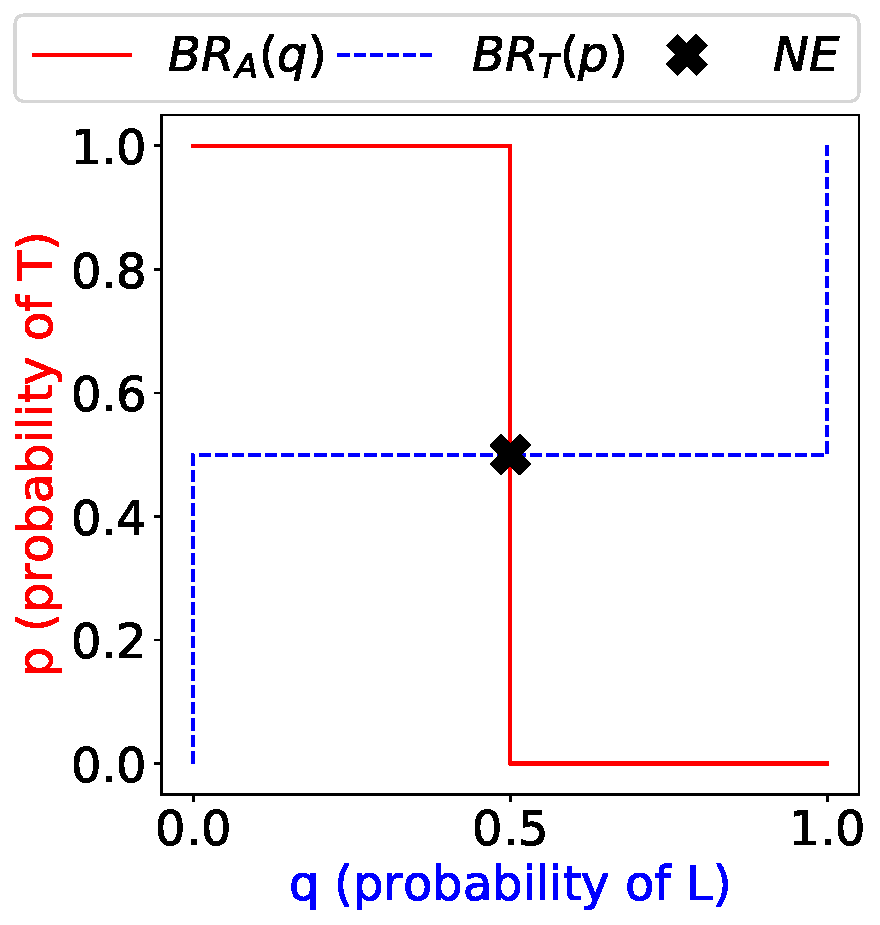
\includegraphics[width=\columnwidth]{figures/3b}
    The only NE is the Mixed Strategy NE:
    \begin{align*}
      (p^{*},q^{*})=\left(\frac{1}{2},\frac{1}{2}\right)
    \end{align*}
  \vfill\null
  \end{multicols}
\end{frame}
\begin{frame}{PS4, Ex. 3.c: The Focal Point}
  \begin{multicols}{2}
    \begin{itemize}
      \item[(c)] Now assume again that Thomas and Alice both want to meet (so that payoffs are as in part (a)), but now there are $N$ bars in town, where $N$ can be very large. Show that there are $2^N-1$ equilibria (pure and mixed). Say that the bars have names: “The First Bar in Town”, “The Second Bar in Town”, and so on. Which equilibrium is the most realistic?
    \end{itemize}
  \vfill\null \columnbreak
    \textit{See "Problem Set 3 Solutions", ex. 8}
  \vfill\null
  \end{multicols}
\end{frame}


\section{PS4, Ex. 4: Generalized Battle of the Sexes}

\begin{frame}{PS4, Ex. 4: Generalized Battle of the Sexes}
  \begin{multicols}{2}
    Consider the following Generalized Battle of the Sexes game, with $N > 1$:
    \begin{table}
      \begin{tabular}{cl|c|c|}
          & \multicolumn{1}{c}{} & \multicolumn{2}{c}{Player 2}\\
          \parbox[t]{1mm}{\multirow{3}{*}{\rotatebox[origin=r]{90}{Player 1}}}
          & \multicolumn{1}{c}{} & \multicolumn{1}{c}{C1 (q)} & \multicolumn{1}{c}{C2 (1-q)} \\\cline{3-4}
          & C1 (p)    & N, 1 & 0, 0 \\\cline{3-4}
          & C2 (1-p)  & 0, 0 & 1, N \\\cline{3-4}
      \end{tabular}
    \end{table}
  \vfill\null \columnbreak
    \begin{itemize}
      \item[(a)] How can you interpret the parameter $N$?
      \item[(b)] Solve for the mixed strategy Nash equilibrium (MSNE). When $N$ becomes very large, what happens to the probability of successful coordination?
    \end{itemize}
  \vfill\null
  \end{multicols}
\end{frame}
\begin{frame}{PS4, Ex. 4: Generalized Battle of the Sexes}
  \begin{multicols}{2}
    \begin{table}
      \begin{tabular}{cl|c|c|}
          & \multicolumn{1}{c}{} & \multicolumn{2}{c}{\color{blue}Player 2}\\
          \parbox[t]{1mm}{\multirow{3}{*}{\rotatebox[origin=r]{90}{\color{red}Player 1}}}
          & \multicolumn{1}{c}{} & \multicolumn{1}{c}{C1 (q)} & \multicolumn{1}{c}{C2 (1-q)} \\\cline{3-4}
          & C1 (p)    & \textcolor{red}{N}, \textcolor{blue}{1} & 0, 0 \\\cline{3-4}
          & C2 (1-p)  & 0, 0 & \textcolor{red}{1}, \textcolor{blue}{N} \\\cline{3-4}
      \end{tabular}
    \end{table}
    \begin{itemize}
      \item[(a)] How can you interpret the $N$?
    \end{itemize}
    \begin{itemize}
      \item[(b)] Solve for the MSNE.
    \end{itemize}
    \vspace{-8pt}
    \begin{align*}
      BR_1(q)=\left\{ \begin{array}{lcl}
          p=0       & \text{if} & q<\frac{1}{1+N} \\
          p\in[0,1] & \text{if} & q=\frac{1}{1+N} \\
          p=1       & \text{if} & q>\frac{1}{1+N}
      \end{array}\right. \\
      BR_2(p)=\left\{ \begin{array}{lcl}
          q=1       & \text{if} & p<\frac{N}{1+N}  \\
          q\in[0,1] & \text{if} & p=\frac{N}{1+N} \\
          q=0       & \text{if} & p>\frac{N}{1+N}
      \end{array}\right.
    \end{align*}
    \begin{align*}
      NE:(p^{*},q^{*})=\left\{(0,0);(1,1);\left(\frac{1}{2},\frac{1}{2}\right)\right\}
    \end{align*}
  \vfill\null \columnbreak
    (example plot for $N=1$)
    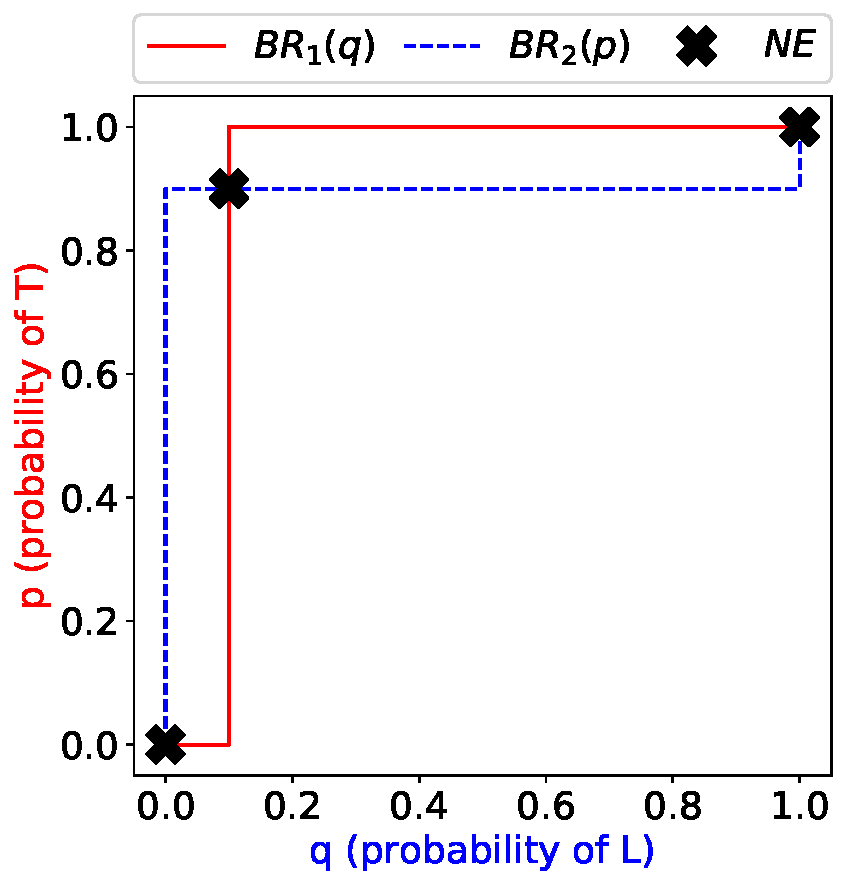
\includegraphics[width=\columnwidth]{figures/4b}
    \vspace{-0pt}
    When $N\rightarrow\infty$, what happens to the probability of successful coordination?
  \vfill\null
  \end{multicols}
\end{frame}


\section{PS4, Ex. 5: North-Atlantic, 1943}

\begin{frame}{PS4, Ex. 5: North-Atlantic, 1943}
  North-Atlantic, 1943. An allied convoy, counting 100 ships, is heading east and it can choose between a northern route where icebergs are known to be numerous or a more southern route. The northern route is dangerous - because of the icebergs - and it is estimated that 6 ships will get lost due to icebergs. Below the surface, the wolf-pack lures. If the u-boats catch the convoy on the southern route, it is a field day, and 40 ships from the convoy are estimated to get lost. If the u-boats catch the convoy on the northern route, they do not have as much time hunting down the convoy - due to petrol shortages - and they are only expected to be able to sink 20 ships from the convoy. The wolf-pack does not have time to check both locations, north and south. Each headquarter (allied or nazi) has to decide whether to go north or south. Unfortunately, there is no radar etc, so one cannot observe the move of the enemy before taking a decision. Each headquarter has a simple payoff function. For the allied headquarter it equals the number of ships making it across the Atlantic. For the nazi headquarter payoff equals the number of ships lost by the allies.
  \begin{itemize}
    \item[(a)] Write down this strategic situation in a bi-matrix.
    \item[(b)] Find the Nash Equilibrium (equilibria?)
    \item[(c)] In equilibrium, what is the expected number of ships that make it across the Atlantic?
  \end{itemize}
\end{frame}
\begin{frame}{PS4, Ex. 5: North-Atlantic, 1943}
    \begin{itemize}
      \item[(a)] It's a zero-sum (100-sum) type game:
    \end{itemize}
    \vspace{-15pt}
    \hspace{-15pt}\begin{table}
      \begin{tabular}{cl|c|c|}
          & \multicolumn{1}{c}{} & \multicolumn{2}{c}{\color{blue}Nazis}\\
          \parbox[t]{1mm}{\multirow{3}{*}{\rotatebox[origin=r]{90}{\color{red}Allied}}}
          & \multicolumn{1}{c}{} & \multicolumn{1}{c}{North (q)} & \multicolumn{1}{c}{South (1-q)} \\\cline{3-4}
          & North (p)    & 74, \textcolor{blue}{26} & \textcolor{red}{94}, 6 \\\cline{3-4}
          & South (1-p)  & \textcolor{red}{100}, 0 & 60, \textcolor{blue}{40} \\\cline{3-4}
      \end{tabular}
    \end{table}
    \begin{itemize}
      \item[(b)] There are no PSNE, find the MSNE:
    \end{itemize}
    The Allied are indifferent for:
    \begin{align*}
      E[u_A|North]&=E[u_A|South]\\
      74q + 94(1-q) &= 100q + 60(1-q) \Rightarrow q = \frac{17}{30}
    \end{align*}
    The Nazis are indifferent for:
    \begin{align*}
      E[u_N|North]&=E[u_N|South]\\
      26p &= 6p + 40(1-p) \Rightarrow q = \frac{2}{3}
    \end{align*}
    \begin{align*}
      \Rightarrow NE=(p^{*},q^{*})=\left(\frac{2}{3},\frac{17}{30}\right)
    \end{align*}
\end{frame}
\begin{frame}{PS4, Ex. 5: North-Atlantic, 1943}
  \begin{itemize}
    \item[(c)] In equilibrium, the expected number of ships that make it across the Atlantic:
  \end{itemize}
  \begin{align*}
     u_A(p^{*},q^{*}) &= p^{*}u_A(North)+(1-p^{*})u_A(South)\\
     &= \frac{2}{3}(74q + 94(1-q)) + \left(1-\frac{2}{3}\right)(100q + 60(1-q))
     &= \vdots \\
     &\approx 82.67
  \end{align*}
\end{frame}


\section{PS4, Ex. 6: Stopping the bike thief}

\begin{frame}{PS4, Ex. 6: Stopping the bike thief}
  \begin{multicols}{2}
    As in Problem Set 2, there are $N\geq2$ people observing someone trying to steal a parked bike. Each of the witnesses would like the thief to be stopped, but prefers not to do it him/herself (because it is unpleasant and perhaps even dangerous). More precisely, if the thief is stopped by someone else, each of the witnesses gets a utility of $v > 0$. Every person who stops the thief gets a utility of $v-c>0$, where $c$ is the cost of interaction with the thief. Finally, if nobody stops the thief and the bike gets stolen, every witness gets a utility of $0$. The witnesses decide whether or not to stop the thief simultaneously and independently.
  \vfill\null \columnbreak
    \begin{itemize}
      \item[a)] Solve for a symmetric mixed strategy equilibrium of this game, where each witness stops the thief with probability $p\in(0,1)$.
      \item[b)] Discuss what happens to $p$ as the number of witness becomes very large. What happens then to the probability that the thief will get stopped? What is the intuition for this result?
    \end{itemize}
    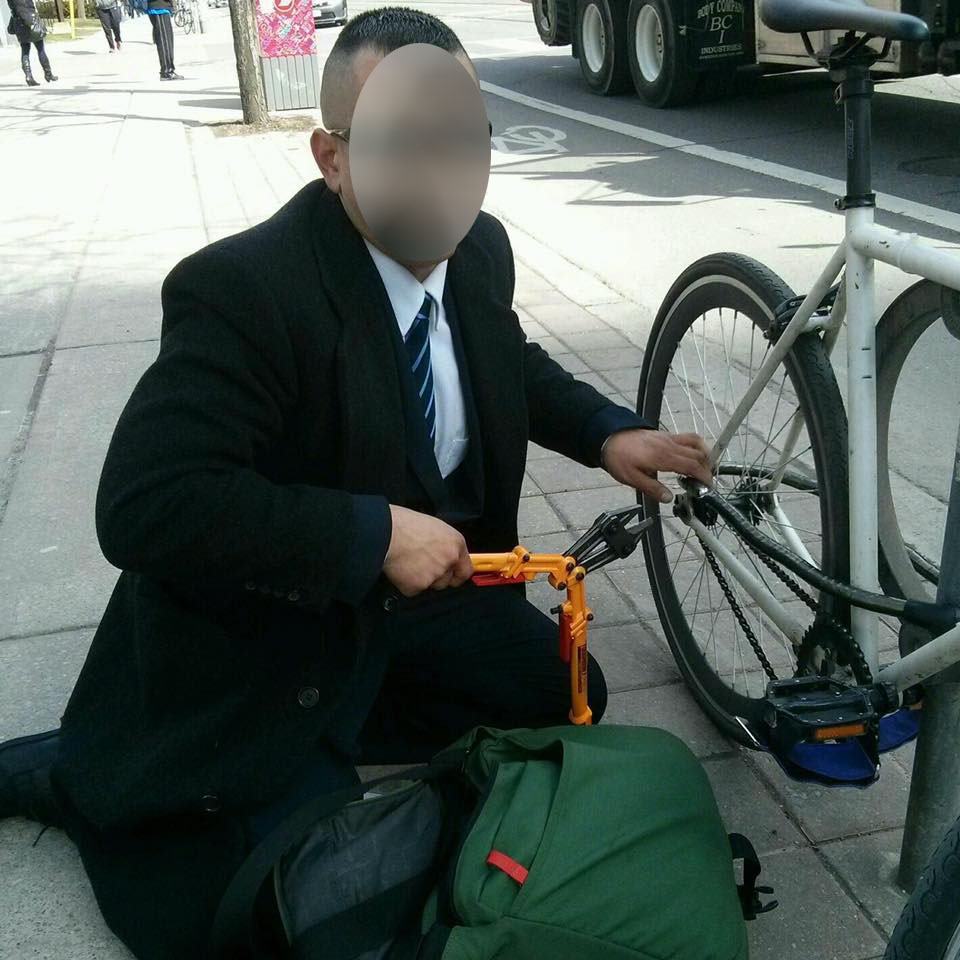
\includegraphics[width=\columnwidth]{figures/bike_thief}
  \vfill\null
  \end{multicols}
\end{frame}
\begin{frame}{PS4, Ex. 6: Stopping the bike thief}
    \begin{itemize}
      \item[a)] Solve for a symmetric mixed strategy equilibrium of this game, where each witness stops the thief with probability $p\in(0,1)$.
    \end{itemize}
    \begin{itemize}
      \item[b)] Discuss what happens to $p$ as the number of witness becomes very large. What happens then to the probability that the thief will get stopped? What is the intuition for this result?
    \end{itemize}
\end{frame}


\section{PS4, Ex. 7: To split or not to split (game tree)}

\begin{frame}{PS4, Ex. 7: To split or not to split}
  \begin{multicols}{2}
    Consider the following 2 × 2 game where payoffs are monetary:
    \begin{table}
      \begin{tabular}{cl|c|c|}
          & \multicolumn{1}{c}{} & \multicolumn{2}{c}{Player 2}\\
          \parbox[t]{1mm}{\multirow{3}{*}{\rotatebox[origin=r]{90}{Player 1}}}
          & \multicolumn{1}{c}{} & \multicolumn{1}{c}{L} & \multicolumn{1}{c}{R} \\\cline{3-4}
          & T & 3, 3 & 0, 4 \\\cline{3-4}
          & B & 4, 0 & 1, 1 \\\cline{3-4}
      \end{tabular}
    \end{table}
    Before this game is played, Player 1 can choose whether, after the game is played, players should keep their own payoffs or split the aggregate payoff evenly between them.
  \vfill\null \columnbreak
    \begin{itemize}
      \item[(a)] Draw the game tree of this two-stage game (assuming that Players 1’s choice of whether to split payoffs is revealed to Player 2 before the second stage).
      \item[(b)] Solve by backwards induction.
    \end{itemize}
  \vfill\null
  \end{multicols}
\end{frame}
\begin{frame}{PS4, Ex. 7: To split or not to split}
  \begin{multicols}{2}
    Consider the following 2 × 2 game where payoffs are monetary:
    \begin{table}
      \begin{tabular}{cl|c|c|}
          & \multicolumn{1}{c}{} & \multicolumn{2}{c}{Player 2}\\
          \parbox[t]{1mm}{\multirow{3}{*}{\rotatebox[origin=r]{90}{Player 1}}}
          & \multicolumn{1}{c}{} & \multicolumn{1}{c}{L} & \multicolumn{1}{c}{R} \\\cline{3-4}
          & T & 3, 3 & 0, 4 \\\cline{3-4}
          & B & 4, 0 & 1, 1 \\\cline{3-4}
      \end{tabular}
    \end{table}
    Before this game is played, Player 1 can choose whether, after the game is played, players should keep their own payoffs or split the aggregate payoff evenly between them.
  \vfill\null \columnbreak
    \begin{itemize}
      \item[(a)] Draw the game tree of this two-stage game (assuming that Players 1’s choice of whether to split payoffs is revealed to Player 2 before the second stage).
      \item[(b)] Solve by backwards induction.
    \end{itemize}
  \vfill\null
  \end{multicols}
\end{frame}


\section{PS3, Ex. 5: Luxembourg as a rogue state}

\begin{frame}{PS3, Ex. 5: Luxembourg as a rogue state}
  \begin{multicols}{2}
    Assume that Luxembourg has turned into a rogue state. It is close to acquiring nuclear weapons, which would threaten the stability in the whole region. The Vatican ($V$) and Denmark ($D$) are preparing an attack on Luxembourg’s nuclear research facilities to stop or slow down its nuclear program. The probability that the attack will be a success is
    \begin{align*}
      p(s_V,s_D)=s_V+s_D-s_vs_D,
    \end{align*}
    where $s_i\in[0,1]$ is the share of its military capacity that country $i\ (i\in\{V,D\})$ uses in the attack. If the attack is successful then each country receives a payoff of 1. The cost of participating in the attack for country $i$ is
    \begin{align*}
      c_i(s_i)=s_i^2
    \end{align*}
    The objective of each country is to maximize its expected payoff from the attack minus the cost.
  \vfill\null\columnbreak
    \begin{itemize}
      \item[(a)] Suppose that the Vatican and Denmark choose the shares of military capacity to use in the attack simultaneously and independently. Find the Nash equilibrium (NE) of this game.
      \item[(b)] Find the social optimum (SO) under the condition that the two countries use the same share of their military capacity. I.e., find the $\bar{s}_V=\bar{s}_D=\bar{s}$ that maximizes aggregate payoff from the attack minus costs. Compare with the equilibrium from question (a) and give an intuitive explanation of your findings.
    \end{itemize}
    \hfill 
\includegraphics[width=0.20 \textwidth]{figures/nuclear}
  \vfill\null
  \end{multicols}
\end{frame}
\begin{frame}{PS3, Ex. 5: Luxembourg as a rogue state}
  \begin{multicols}{2}
    \begin{itemize}
      \item[(a)] Find the NE in the static game:
    \end{itemize}
    Expected payoff for player $i\neq j$:
    \begin{align*}
      u_i(s_i,s_j)=\underbrace{s_i+s_j-s_is_j}_\text{Probability of success}-\underbrace{s_i^2}_\text{Cost}
    \end{align*}
  \vfill\null\columnbreak
  \vfill\null
  \end{multicols}
\end{frame}
\begin{frame}{PS3, Ex. 5: Luxembourg as a rogue state}
  \begin{multicols}{2}
    \begin{itemize}
      \item[(a)] Find the NE in the static game:
    \end{itemize}
    Expected payoff for player $i\neq j$:
    \begin{align*}
      u_i(s_i,s_j)=\underbrace{s_i+s_j-s_is_j}_\text{Probability of success}-\underbrace{s_i^2}_\text{Cost}
    \end{align*}
    Find the best-response function for $i$:
    \begin{align*}
      FOC:\ \frac{\delta u_i}{\delta s_i}=1+0-s_j-2s_i&=0\\
       s_i&=\frac{1-s_j}{2}
    \end{align*}
  \vfill\null\columnbreak
  \vfill\null
  \end{multicols}
\end{frame}
\begin{frame}{PS3, Ex. 5: Luxembourg as a rogue state}
  \begin{multicols}{2}
    \begin{itemize}
      \item[(a)] Find the NE in the static game:
    \end{itemize}
    Expected payoff for player $i\neq j$:
    \begin{align*}
      u_i(s_i,s_j)=\underbrace{s_i+s_j-s_is_j}_\text{Probability of success}-\underbrace{s_i^2}_\text{Cost}
    \end{align*}
    Find the best-response function for $i$:
    \begin{align*}
      FOC:\ \frac{\delta u_i}{\delta s_i}=1+0-s_j-2s_i&=0\\
       s_i&=\frac{1-s_j}{2}
    \end{align*}
    Taking advantage of symmetry $s_i^{*}=s_j^{*}$:
    \begin{align*}
       s_i^{*}&=\frac{1-s_i^{*}}{2}\\
      2s_i^{*}+s_i^{*}&=1\\
       s_i^{*}&=\frac{1}{3}\equiv s^{NE}
    \end{align*}
    i.e. $NE=\left\{(s_D^{*},s_V^{*})=(\frac{1}{3},\frac{1}{3})\right\}$
  \vfill\null\columnbreak
  \vfill\null
  \end{multicols}
\end{frame}
\begin{frame}{PS3, Ex. 5: Luxembourg as a rogue state}
  \begin{multicols}{2}
    \begin{itemize}
      \item[(a)] Find the NE in the static game:
    \end{itemize}
    Expected payoff for player $i\neq j$:
    \begin{align*}
      u_i(s_i,s_j)=\underbrace{s_i+s_j-s_is_j}_\text{Probability of success}-\underbrace{s_i^2}_\text{Cost}
    \end{align*}
    Find the best-response function for $i$:
    \begin{align*}
      FOC:\ \frac{\delta u_i}{\delta s_i}=1+0-s_j-2s_i&=0\\
       s_i&=\frac{1-s_j}{2}
    \end{align*}
    Taking advantage of symmetry $s_i^{*}=s_j^{*}$:
    \begin{align*}
       s_i^{*}&=\frac{1-s_i^{*}}{2}\\
      2s_i^{*}+s_i^{*}&=1\\
       s_i^{*}&=\frac{1}{3}\equiv s^{NE}
    \end{align*}
    i.e. $NE=\left\{(s_D^{*},s_V^{*})=(\frac{1}{3},\frac{1}{3})\right\}$
  \vfill\null\columnbreak
    \begin{itemize}
      \item[(b)] Find the SO given shares are equal:
    \end{itemize}
  \vfill\null
  \end{multicols}
\end{frame}
\begin{frame}{PS3, Ex. 5: Luxembourg as a rogue state}
  \begin{multicols}{2}
    \begin{itemize}
      \item[(a)] Find the NE in the static game:
    \end{itemize}
    Expected payoff for player $i\neq j$:
    \begin{align*}
      u_i(s_i,s_j)=\underbrace{s_i+s_j-s_is_j}_\text{Probability of success}-\underbrace{s_i^2}_\text{Cost}
    \end{align*}
    Find the best-response function for $i$:
    \begin{align*}
      FOC:\ \frac{\delta u_i}{\delta s_i}=1+0-s_j-2s_i&=0\\
       s_i&=\frac{1-s_j}{2}
    \end{align*}
    Taking advantage of symmetry $s_i^{*}=s_j^{*}$:
    \begin{align*}
       s_i^{*}&=\frac{1-s_i^{*}}{2}\\
      2s_i^{*}+s_i^{*}&=1\\
       s_i^{*}&=\frac{1}{3}\equiv s^{NE}
    \end{align*}
    i.e. $NE=\left\{(s_D^{*},s_V^{*})=(\frac{1}{3},\frac{1}{3})\right\}$
  \vfill\null\columnbreak
    \begin{itemize}
      \item[(b)] Find the SO given shares are equal:
    \end{itemize}
    Expected payoff for $i$, $\bar{s}_D=\bar{s}_V=\bar{s}$:
    \begin{align*}
      u_i(\bar{s})&=\underbrace{\bar{s}+\bar{s}-\bar{s}\bar{s}}_\text{Probability of success}-\underbrace{\bar{s}^2}_\text{Cost}\\
                  &=2\bar{s}-2\bar{s}^2
    \end{align*}
  \vfill\null
  \end{multicols}
\end{frame}
\begin{frame}{PS3, Ex. 5: Luxembourg as a rogue state}
  \begin{multicols}{2}
    \begin{itemize}
      \item[(a)] Find the NE in the static game:
    \end{itemize}
    Expected payoff for player $i\neq j$:
    \begin{align*}
      u_i(s_i,s_j)=\underbrace{s_i+s_j-s_is_j}_\text{Probability of success}-\underbrace{s_i^2}_\text{Cost}
    \end{align*}
    Find the best-response function for $i$:
    \begin{align*}
      FOC:\ \frac{\delta u_i}{\delta s_i}=1+0-s_j-2s_i&=0\\
       s_i&=\frac{1-s_j}{2}
    \end{align*}
    Taking advantage of symmetry $s_i^{*}=s_j^{*}$:
    \begin{align*}
       s_i^{*}&=\frac{1-s_i^{*}}{2}\\
      2s_i^{*}+s_i^{*}&=1\\
       s_i^{*}&=\frac{1}{3}\equiv s^{NE}
    \end{align*}
    i.e. $NE=\left\{(s_D^{*},s_V^{*})=(\frac{1}{3},\frac{1}{3})\right\}$
  \vfill\null\columnbreak
    \begin{itemize}
      \item[(b)] Find the SO given shares are equal:
    \end{itemize}
    Expected payoff for $i$, $\bar{s}_D=\bar{s}_V=\bar{s}$:
    \begin{align*}
      u_i(\bar{s})&=\underbrace{\bar{s}+\bar{s}-\bar{s}\bar{s}}_\text{Probability of success}-\underbrace{\bar{s}^2}_\text{Cost}\\
                  &=2\bar{s}-2\bar{s}^2
    \end{align*}
    Social planner target function:
    \begin{align*}
      \pi^S(\bar{s})&=\underbrace{2}_\text{Countries}(2\bar{s}-2\bar{s}^2)=4\bar{s}-4\bar{s}^2
    \end{align*}
  \vfill\null
  \end{multicols}
\end{frame}
\begin{frame}{PS3, Ex. 5: Luxembourg as a rogue state}
  \begin{multicols}{2}
    \begin{itemize}
      \item[(a)] Find the NE in the static game:
    \end{itemize}
    Expected payoff for player $i\neq j$:
    \begin{align*}
      u_i(s_i,s_j)=\underbrace{s_i+s_j-s_is_j}_\text{Probability of success}-\underbrace{s_i^2}_\text{Cost}
    \end{align*}
    Find the best-response function for $i$:
    \begin{align*}
      FOC:\ \frac{\delta u_i}{\delta s_i}=1+0-s_j-2s_i&=0\\
       s_i&=\frac{1-s_j}{2}
    \end{align*}
    Taking advantage of symmetry $s_i^{*}=s_j^{*}$:
    \begin{align*}
       s_i^{*}&=\frac{1-s_i^{*}}{2}\\
      2s_i^{*}+s_i^{*}&=1\\
       s_i^{*}&=\frac{1}{3}\equiv s^{NE}
    \end{align*}
    i.e. $NE=\left\{(s_D^{*},s_V^{*})=(\frac{1}{3},\frac{1}{3})\right\}$
  \vfill\null\columnbreak
    \begin{itemize}
      \item[(b)] Find the SO given shares are equal:
    \end{itemize}
    Expected payoff for $i$, $\bar{s}_D=\bar{s}_V=\bar{s}$:
    \begin{align*}
      u_i(\bar{s})&=\underbrace{\bar{s}+\bar{s}-\bar{s}\bar{s}}_\text{Probability of success}-\underbrace{\bar{s}^2}_\text{Cost}\\
                  &=2\bar{s}-2\bar{s}^2
    \end{align*}
    Social planner target function:
    \begin{align*}
      \pi^S(\bar{s})&=\underbrace{2}_\text{Countries}(2\bar{s}-2\bar{s}^2)=4\bar{s}-4\bar{s}^2
    \end{align*}
    Find the social optimum (SO):
    \begin{align*}
      FOC:\ \frac{\delta\pi^S}{\delta s_i}=4-8\bar{S}&=0\\
       \bar{S}&=\frac{4}{8}=\frac{1}{2}>\frac{1}{3}
    \end{align*}
    i.e. the SO is higher than the NE as the positive externality is not rewarded, leading to an incentive to free ride.
  \vfill\null
  \end{multicols}
\end{frame}


\section{PS4, Ex. 8: Building a playground (Stackelberg)}

\begin{frame}{PS4, Ex. 8: Building a playground (Stackelberg)}
  \begin{multicols}{2}
    Two neighbors are building a common playground for their children. The time spent on the project by neighbor $i$ is $x_i \geq 0,\ i = 1, 2$. The resulting quality of the playground is
    \begin{align*}
      q(x_1,x_2)=x_1+x_2-x_1x_2
    \end{align*}
    Spending time on the project is costly. More precisely, the cost function of the neighbors are:
    \begin{align*}
      C_i(x_i)=x_i^2,\ \ \ i=1,2
    \end{align*}
    The payoff of neighbor $i$, $U_i$, is equal to the quality of the playground minus his cost.
    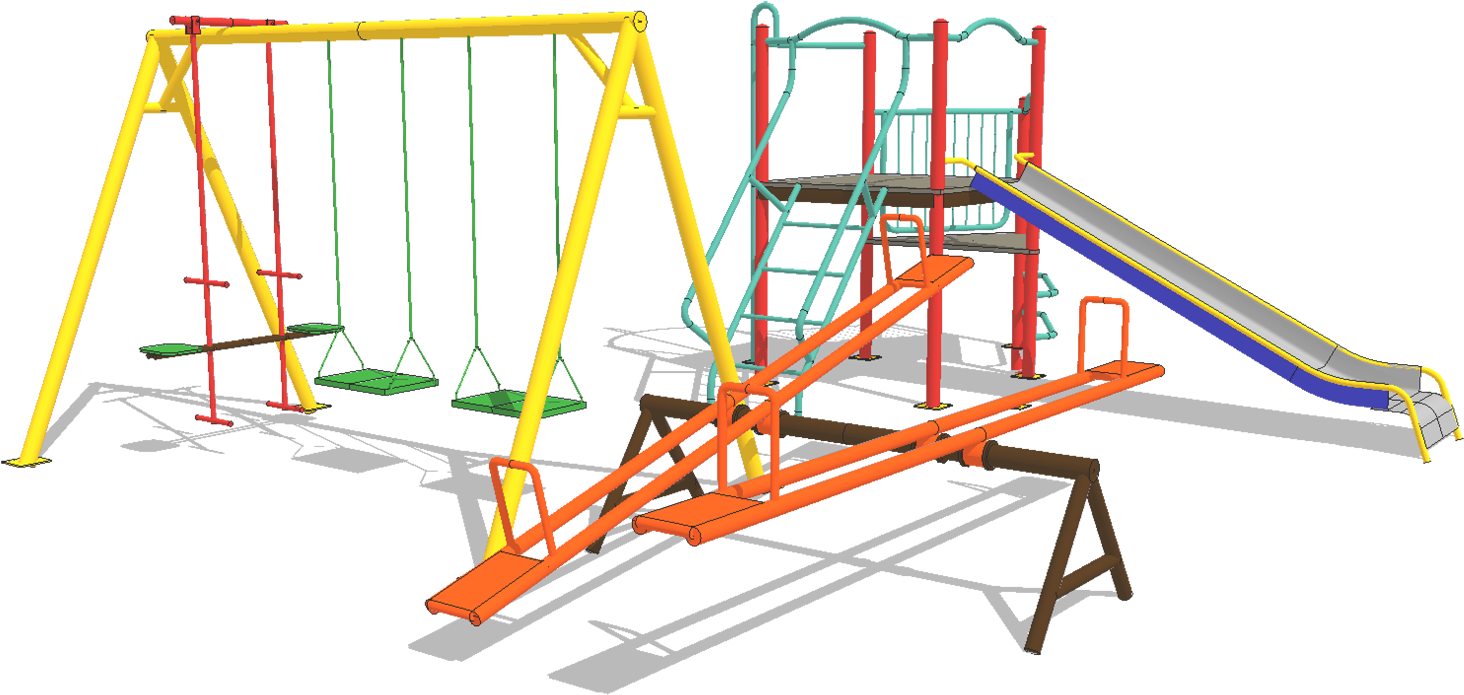
\includegraphics[width=\columnwidth]{figures/playground}
  \vfill\null \columnbreak
    \begin{itemize}
      \item[(a)] Suppose the neighbors decide how much time to spend on the project simultaneously and independently. Derive the best response functions. Find the Nash equilibrium of this game.
      \item[(b)] Suppose now that the game is played in two stages. First, neighbor 1 decides how much time to spend on the project. Neighbor 2 observes this and then chooses how much time to put in himself. Find the backwards induction outcome of this game.
      \item[(c)] Compare the games from (a) and (b) with respect to the payoff that each neighbor obtains. Give an intuitive explanation of your results.
    \end{itemize}
  \vfill\null
  \end{multicols}
\end{frame}
\begin{frame}{PS4, Ex. 8: Building a playground (Stackelberg)}
  \begin{multicols}{2}
    \begin{itemize}
      \item[(a)] Suppose the neighbors decide how much time to spend on the project simultaneously and independently. Derive the best response functions. Find the Nash equilibrium of this game.
    \end{itemize}
  \vfill\null \columnbreak
    \begin{itemize}
      \item[(b)] Suppose now that the game is played in two stages. First, neighbor 1 decides how much time to spend on the project. Neighbor 2 observes this and then chooses how much time to put in himself. Find the backwards induction outcome of this game.
    \end{itemize}
    \begin{itemize}
      \item[(c)] Compare the games from (a) and (b) with respect to the payoff that each neighbor obtains. Give an intuitive explanation of your results.
    \end{itemize}
  \vfill\null
  \end{multicols}
\end{frame}



% \section{PS4, Ex. : }
%
% \begin{frame}{PS4, Ex. : }
%   \begin{multicols}{2}
%   \vfill\null \columnbreak
%   \vfill\null
%   \end{multicols}
% \end{frame}


% \section{PS4, Ex. : }
%
% \begin{frame}{PS4, Ex. : }
%   \begin{multicols}{2}
%     \begin{table}
%       \begin{tabular}{cl|c|c|}
%           & \multicolumn{1}{c}{} & \multicolumn{2}{c}{Player 2}\\
%           \parbox[t]{1mm}{\multirow{3}{*}{\rotatebox[origin=r]{90}{Player 1}}}
%           & \multicolumn{1}{c}{} & \multicolumn{1}{c}{L (q)} & \multicolumn{1}{c}{R (1-q)} \\\cline{3-4}
%           & T (p)   &  &  \\\cline{3-4}
%           & B (1-p) &  &  \\\cline{3-4}
%       \end{tabular}
%     \end{table}
%   \vfill\null \columnbreak
%     \begin{table}
%       \begin{tabular}{cc|c|c|}
%         & \multicolumn{1}{c}{} & \multicolumn{2}{c}{\color{blue}Player 2}\\
%         \parbox[t]{1mm}{\multirow{3}{*}{\rotatebox[origin=r]{90}{\color{red}Player 1}}}
%         & \multicolumn{1}{c}{} & \multicolumn{1}{c}{L (q)} & \multicolumn{1}{c}{R (1-q)} \\\cline{3-4}
%         & T (p)   & \textcolor{red}{}, \textcolor{blue}{} &   \\\cline{3-4}
%         & B (1-p) &  &  \\\cline{3-4}
%       \end{tabular}
%     \end{table}
%     \begin{table}
%       \begin{tabular}{l|c|c|}
%           \multicolumn{1}{c}{} & \multicolumn{1}{c}{L (q)} & \multicolumn{1}{c}{L (1-q)} \\\cline{2-3}
%           T (p)   &  &  \\\cline{2-3}
%           B (1-p) &  &  \\\cline{2-3}
%       \end{tabular}
%     \end{table}
%   \vfill\null
%   \end{multicols}
% \end{frame}


\end{document}
